\documentclass[11pt]{article}
\usepackage[framemethod=TikZ]{mdframed}
\usepackage{amsthm}
\usepackage{tcolorbox}
\usepackage[legalpaper, margin=1in]{geometry}
\usepackage{setspace}
\usepackage{amsmath}
\usepackage{cancel}
\usepackage{multicol}
\def\deg{\ensuremath{^\circ}}
\def\v#1{\ensuremath{\mathrm{#1}}}
\usepackage{multirow}
\usepackage{fancyhdr}
\pagestyle{fancy}
\usepackage{lastpage} 
\usepackage{colortbl}
\usepackage{amssymb}
\usepackage{graphicx}
\setlength{\parskip}{0pt}
\lhead{Jhon Christian N. Rozano}
\chead{}
\rhead{April 10, 2021}

\lfoot{Sources: MATH Mental Abuse To Human, Brilliant}
\cfoot{}
\rfoot{Page \thepage\ of \pageref{LastPage}}

\renewcommand{\headrulewidth}{1pt}

\renewcommand{\footrulewidth}{1pt}

\newcommand*\Eval[3]{\left.#1\right\rvert_{#2}^{#3}}

\definecolor{LightCyan}{rgb}{0.88,1,1}



\begin{document}
	\setlength{\columnsep}{10pt}
	\renewcommand{\arraystretch}{1.5}
	\singlespacing
	
	\begin{center}
		{\large  \textbf{Math Problem of the Day}} \\ 
	\end{center}
	
	\noindent Evaluate the integral
	\[ \int \frac{1}{x\sqrt{x^{69}-1}} \, dx \]
	
	\newtcolorbox{mybox}[1]{title=#1}
	\begin{mybox}{\textbf{Solution}}
			Let \( u^2 = x^{69} - 1 \), then we have \( 2u \, du = 69x^{68} \, dx \)
			\[ dx = \frac{2u}{69x^{68}} \, du \Rightarrow \int \frac{1}{x\sqrt{x^{69}-1}} \cdot \frac{2u}{69x^{68}} \, du = \int \frac{1}{x \cdot u } \cdot \frac{2u}{69x^{68}} \, du \] 
			\[ \frac{2}{69} \int \frac{u}{u \cdot x^{69}} \, du = \frac{2}{69} \int \frac{1}{x^{69}} \, du   \]
			Since \( u^2 = x^{69} - 1 \), we know that \( x^{69} = u^2 + 1  \). Then the integral becomes
			\[ \frac{2}{69} \int \frac{1}{u^2+1} \, du    \]
			Notice that the integral of  \( \frac{1}{u^2+1} \) is equal to the derivative of \( \text{tan}^{-1} u  \)
			Therefore 
			\[ \frac{2}{69} \int \frac{1}{u^2+1} \, du = \frac{2}{69} \cdot \text{tan}^{-1} u + \text{C} = \boxed{\frac{2}{69} \cdot \text{tan}^{-1}{\sqrt{x^{69}-1}} + \text{C}} \]	
	\end{mybox}
	\bigskip
	\begin{center}
		{\large  \textbf{Physics Problem of the Day}} \\ 
	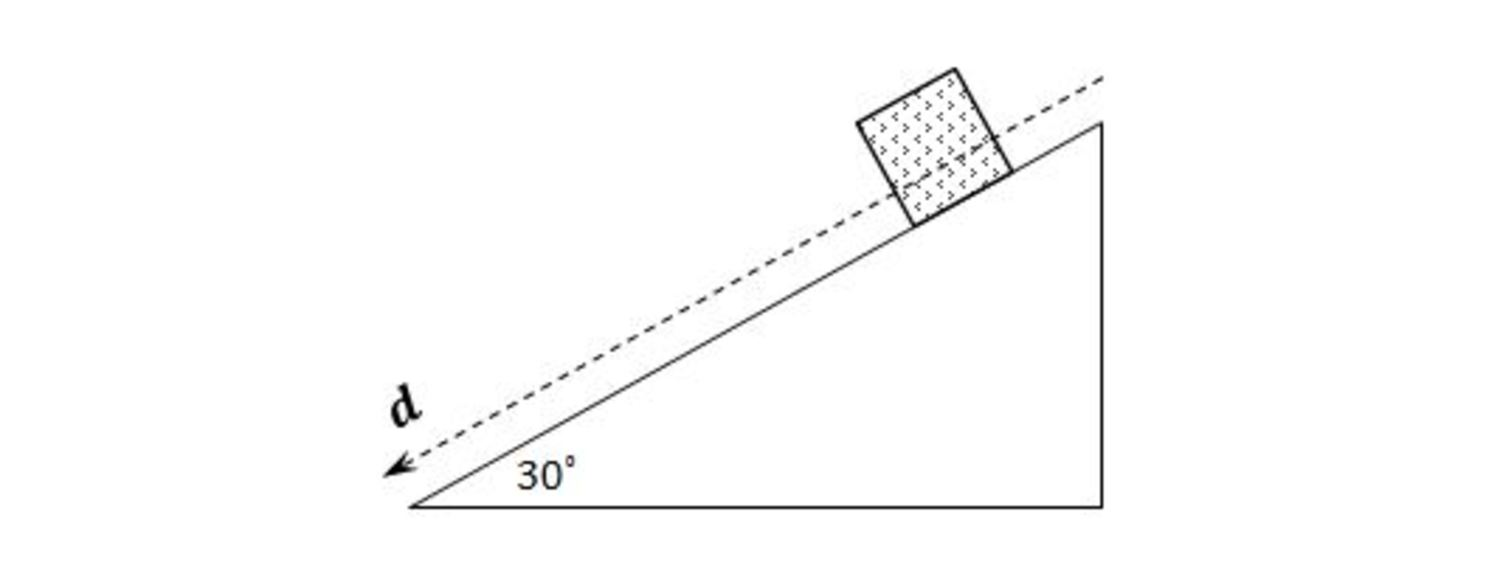
\includegraphics[clip=true, scale=0.2, trim=0mm 0mm 0mm 0mm]{bdc8e6790a.1034f968f4.G13Xge.jpg}
	\end{center}
	\noindent The above diagram depicts a ramp of distance $d=10\text{ m}$ with an incline angle of 30$\deg$.  A box with mass $m=25\text{ kg}$ is sliding down the inclined plane and the coefficient of kinetic friction between the box and the ramp is $\mu_k=0.2$. What is the total work done on the box by all of the forces acting on it? \\
	
	\noindent The gravitational acceleration is $g = 10 \, m/s^2$
	\begin{mybox}{\textbf{Solution}}
		Note that the forces acting on the box are gravitational force \(F_g \), friction force \( f_k \), and normal force \(F_n\). Since the box also sits on the inclined plane, the component of the gravitational force \( F_g \) is parallel to the plane where the box is moving. \\
		
		Hence, the work done by the gravity is given by
		\[ W_g = F \cdot d = (mg \, \text{sin}\theta) d = (25\text{ kg})(10 \, m/s^2)(\text{sin} \, {30\deg})(10\text{ m}) = 1250\text{ J} \]
		
		The normal force is perpendicular to the direction of the box, so \( \theta = 90\deg \). Therefore, the work done by the normal force \( F_n \) is equal to zero. \\
		
		The kinetic friction force \( f_k \) is equal to the other component of the gravitational force multiplied by the coefficient of kinetic friction \( f_k \). The direction of the kinetic friction is opposite to the direction of the box, and this gives us \( \theta = 180\deg \). Thus, the work done by the friction force \( f_k \) is negative. 
		\[ W_k = F \cdot d = - (\mu mg \, cos\theta) d = (0.2)(25\text{ kg})(10 \, m/s^2)(\text{cos} \, {30\deg})(10\text{ m}) = - 250 \sqrt{3} \text{J} \]
		Therefore, the total work is
		\[ W_{\text{total}} = 1250\text{ J} + (-250\sqrt{3}\text{ J}}) = \boxed{(1250 - 250\sqrt{3})\text{ J}}\]
	\end{mybox}
\end{document}
